\chapter{Modellazione del sistema}
\label{cap:modellazione-sistema}

Questo capitolo fornisce una panoramica riguardo all'infrastruttura del Mobile Edge Computing ed introduce il modello di orchestrazione proposto.


%
%   INFRASTRUTTURA MEC
%
\section{L'infrastruttura Mobile Edge Computing}
\label{sec:infrastruttura-mec}

All'interno di un'infrastruttura Mobile Edge Computing (MEC) si trovano i cluster di virtualizzazione, spesso chiamati `MEC facility' o più semplicemente `facility', e gli access point (AP). Le facility sono il luogo in cui avviene la virtualizzazione, e sono composte dalle macchine virtuali (VM) su cui si eseguono le applicazioni degli utenti finali. Gli AP sono invece i dispositivi (per esempio le antenne wireless) a cui gli end point si collegano per poter ricevere il servizio. Ogni AP è associato ad una facility, a cui inoltra tutto il traffico che riceve: questo significa che ogni facility avrà in esecuzione nelle proprie VM tutte le applicazioni utilizzate dagli utenti connessi agli AP a lui associati.

Data la natura mobile degli end point, che sono per esempio smartphone o laptop, il traffico a cui sono sottoposti gli AP varia nel tempo e di conseguenza cambia la domanda rivolta alle facility. Per questo motivo l'assegnamento viene effettuato dinamicamente, e lo strumento incaricato di tale compito è l'orchestratore, che implementa la logica definita dal modello di orchestrazione. Le azioni che svolge vengono chiamate `orchestrazioni' e consistono nell'assegnare un AP ad una facility diversa da quella attuale, provocando il ridimensionamento della potenza delle VM in termini del numero di processori e memoria utilizzata, e la migrazione del loro stato. Il ridimensionamento è dovuto alla variazione di domanda da soddisfare, mentre la migrazione dello stato è necessaria per avere in esecuzione in ogni facility le applicazioni utilizzate dagli utenti connessi agli AP che le sono assegnati. Il costo prodotto dalla migrazione prende il nome di `costo di migrazione'.

Nel sottocapitolo successivo viene illustrato il modello di orchestrazione proposto in questo lavoro.


%
%   INFRASTRUTTURA MEC
%
\section{Modello di orchestrazione proposto}
\label{sec:modello-di-orchestrazione-proposto}

Il modello di orchestrazione proposto è una variante di quello presentato negli articoli \cite{assignment-patterns}, \cite{analytics-mec} in cui nell'effettuare le scelte di orchestrazione si tiene in considerazione anche l'utilizzo dell'energia da parte delle facility.

Come illustrato in \cite{analytics-mec}, all'interno del modello viene introdotta una discretizzazione temporale che permette di effettuare migrazioni solo in determinati istanti, per esempio ogni 15 minuti. Questa scelta è ragionevole, dato che in caso contrario si pagherebbe un costo troppo elevato in termini di migrazione e spese generali dovute alla gestione del traffico. L'orizzonte temporale viene quindi rappresentato da un insieme di time-slot della stessa durata.

L'obbiettivo del modello è quello di effettuare assegnamenti che permettano di ottenere un buon compromesso tra: una buona qualità del servizio (cioè bassa latenza per l'utente finale), costi di migrazione contenuti e buona gestione dell'energia da parte delle facility. Nell'effettuare le scelte bisogna inoltre tenere in considerazione che la domanda degli AP varia nel corso del tempo e che ogni facility possiede un limite massimo di domanda che è in grado di soddisfare simultaneamente.

Dal punto di vista energetico, le facility utilizzano in ogni slot time una quantità di energia direttamente proporzionale alla domanda complessiva che gli viene rivolta. A tale scopo, ognuna di esse possiede un certo numero di pannelli fotovoltaici che le permettono di generare energia variabile nel tempo, che può essere direttamente utilizzata oppure immagazzinata all'interno delle proprie batterie per i time-slot successivi. Le batterie hanno una capacità limitata e nel caso in cui l'energia prodotta non basti a soddisfare la domanda, è possibile acquistarla ad un prezzo che varia in base all'istante temporale.

\begin{figure}[t]
    \centering
    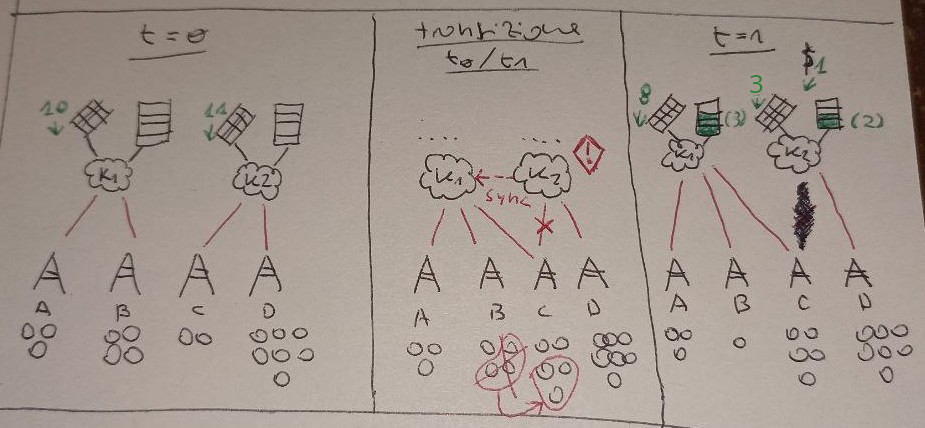
\includegraphics[width = 150mm]{img/example-assigments.jpg}
    \caption{Esempio funzionamento del modello di orchestrazione.}
    \label{fig:esempio-assegnamenti}
\end{figure}


%
%   ESEMPIO FUNZIONAMENTO
%
\subsection{Esempio del funzionamento}
\label{sub-sec:esempio-funzionamento}

Una semplice applicazione di esempio è presentata nella \autoref{fig:esempio-assegnamenti}. Come si può vedere, è presente una rete MEC con due facility (\texttt{K1} e \texttt{K2}) e quattro AP (\texttt{A}, \texttt{B}, \texttt{C}, \texttt{D}) considerata in due time-slot consecutivi (\texttt{t}=0, 1). Gli end point connessi agli AP sono rappresentati con dei piccoli cerchi. Si supponga che in ogni time-slot per gestire la domanda di ogni utente sia necessario utilizzare una singola unità di energia e che inizialmente le batterie siano vuote in entrambe le facility. Nel primo time-slot (\texttt{t}=1) gli AP \texttt{A} e \texttt{B} sono associati alla facility \texttt{K1} mentre \texttt{C} e \texttt{D} a \texttt{K2}, quindi tutti gli utenti che sono connessi ad \texttt{A} e \texttt{B} avranno le proprie applicazioni in esecuzione su una VM presente in \texttt{K1}, mentre quelli connessi a \texttt{C} e \texttt{D} le avranno in \texttt{K2}. Questi assegnamenti permettono di avere una buona latenza, dato che ogni AP è connesso alla facility più vicina, ma anche una buona gestione energetica, in quanto nella facility \texttt{K1} vengono prodotte 10 unità di energia ed utilizzate solo 7 mentre in \texttt{K2} se ne producono 11 e utilizzano 9. In entrambi i casi avanzano delle unità (3 in \texttt{K1} e 2 in \texttt{K2}) che vengono immagazzinate nelle batterie per poter essere spese nei prossivi time-slot. Successivamente tre utenti connessi all'AP \texttt{B} si spostano e vengono agganciati da \texttt{C}: a questo punto \texttt{K2} riceve una richiesta di domanda eccessiva che non riesce a gestire e di conseguenza è necessario effettuare un'azione di orchestrazione per ribilanciare il traffico. Questo comporta assegnare \texttt{C} a \texttt{K1}, ridimensionare le VM (aumentarne la potenza in \texttt{K1} ed abbassarla in \texttt{K2}) e sincronizzare le facility trasferendo lo stato delle VM riguardanti tutti gli utenti connessi a \texttt{C} da \texttt{K2} a \texttt{K1}. In un contesto reale, il modello deve prevenire una situazione di questo tipo effettuando orchestrazioni che tengano in considerazione la futura domanda dei vari AP, dato che questa circostanza va ad inficiare la qualità del servizio offerto. Nel secondo time-slot (\texttt{t}=1) si avranno quindi gli AP \texttt{A}, \texttt{B} e \texttt{C} assegnati alla facility \texttt{K1}, mentre \texttt{D} a \texttt{K2}. Dal punto di vista energetico, la facility \texttt{K1} riesce a soddisfare la domanda di traffico (9 unità) utilizzando l'energia presente nella batteria e quella prodotta in questo time-slot (8 + 3 unità complessive). Per quanto riguarda invece \texttt{K2}, l'energia disponibile (3 + 2 unità) non è sufficiente per colmare la domanda, e quindi è necessario acquistare una ulterione unità. Da notare come l'energia potrebbe avere costi diversi nel corso dei time-slot, e di conseguenza per il modello potrebbe risultare conveniente acquistarla quando il costo è basso per immagazzinarla nelle batterie ed utilizzarla successivamente.


%
%   IMPLEMENTAZIONE
%
\subsection{Implementazione}
\label{sub-sec:implementazione}

Il comportamento del modello di orchestrazione fin qui descritto viene implementato attraverso un modello di programmazione lineare misto-intera (MILP), a cui d'ora in poi ci si riferirà con il nome di `modello completo'. Il modello completo, descritto dettagliatamente nella \autoref{sec:modello-completo}, rappresenta la miglior metodologia per risolvere il problema in quanto garantisce di ottenere la soluzione ottima, ma data la sua natura combinatoria potrebbe essere difficilmente utilizzabile in alcune situazioni. Infatti quando l'arco temporale preso in considerazione oppure il numero di AP e facility tendono ad accrescere, il tempo di calcolo aumenta esponenzialmente fino a diventare proibitivo. 

Per questo motivo vengono successivamente proposte due euristiche che semplificano il problema con l'obbiettivo di abbassare i tempi di calcolo ed ottenere una soluzione non troppo peggiorata rispetto a quella migliore. Nella \autoref{sec:semplificazione-modello} viene rappresentata la prima idea euristica, che consiste nell'utilizzare una semplificazione del modello completo, mentre nella \autoref{sec:aggregamento-time-slot} la seconda, che aggrega i time-slot in modo tale da semplificare l'istanza su cui il modello completo opera.
